\section{Implementace}
V předchozí kapitole jsme diskutovali matematickou úvahu o třídách a jejich skupinách (SubClasses), kde jsme stanovili tři klíčové podmínky: úplnost, disjunkci a podmnožinovou strukturu. V této kapitole se zaměříme na implementaci těchto matematických principů do třídního a databázového modelu. Zároveň se pokusíme najít nejefektivnější řešení, které zajistí plnou konzistenci dat v databázi.

\subsection*{Třídní Model}

Třídní model zahrnuje několik hlavních entit: \texttt{Class}, \texttt{SubClass}, \texttt{Student} a \texttt{StudentAssignment}. Model \texttt{Class} reprezentuje třídu jako celek, model \texttt{SubClass} reprezentuje skupiny v rámci třídy, model \texttt{Student} reprezentuje jednotlivé studenty a model \texttt{StudentAssignment} zaznamenává přiřazení studentů k třídám a skupinám.

\subsubsection*{Class}

\texttt{Class} obsahuje informace o třídě, jako jsou identifikátor třídy, označení třídy, prefix, datum platnosti od a do, místnost a třídní učitel. 

\subsubsection*{SubClass}

\texttt{SubClass} reprezentuje skupiny studentů v rámci třídy. Každá skupina má své vlastní identifikační číslo, název a odkaz na třídu, ke které patří. SubClass může existovat pouze v kontextu třídy, což znamená, že každá SubClass musí být vždy přiřazena konkrétní třídě.

\subsubsection*{Student}

\texttt{Student} obsahuje informace o jednotlivých studentech, jako jsou identifikační číslo, uživatelské jméno, jméno a příjmení.

\subsubsection*{StudentAssignment}

\texttt{StudentAssignment} zaznamenává přiřazení studentů k třídám a skupinám. Obsahuje odkazy na studenty, třídy a skupiny, ke kterým jsou přiřazeni. Klíčovým prvkem tohoto modelu je zajištění trvanlivosti přiřazení, tedy schopnost zaznamenávat změny přiřazení studentů v průběhu roku. 

V průběhu školního roku mohou nastat různé změny, které vyžadují aktualizaci přiřazení studentů. Tyto změny mohou zahrnovat mnoho faktorů a ty nejčastější z nich jsou vyjmenovány níže. Trvanlivost přiřazení umožňuje udržovat historický záznam o všech těchto změnách, což je nezbytné pro správu.

\textbf{Problémy a důvody pro trvanlivost:}

\begin{itemize}
    \item \textbf{Přechody mezi třídami}: Studenti mohou být během školního roku přeřazeni do jiné třídy z různých důvodů, jako jsou změny nálad v třídním kolektivu nebo přestup studenta mezi obory.
    \item \textbf{Změny ve složení skupin}: V závislosti na specifických potřebách výuky mohou být studenti přeřazeni mezi různými skupinami. Například při výuce jazyků může být potřeba změnit složení skupin kvůli homogenizaci, nebo naopak heterogenizaci skupiny, čimž v závislosti na potřebách jednotlivých žáků lze docílit zefektivnění výuky.
\end{itemize}

Model \texttt{StudentAssignment} musí být schopen zaznamenávat všechny tyto změny, aby bylo možné udržovat konzistentní a aktuální přehled o přiřazení studentů. Tento model tedy umožňuje sledování přiřazení studentů k třídám a skupinám v určitém časovém období a zajišťuje, že historické změny jsou správně zaznamenány.

\textbf{Schopnosti modelu:}

\begin{itemize}
    \item \textbf{Referenční integrita}: Každý záznam o přiřazení musí odkazovat na platné záznamy ve třídách a skupinách.
    \item \textbf{Flexibilita přiřazení}: Umožňuje přiřazení studenta buď přímo do třídy nebo do specifické skupiny.
    \item \textbf{Trvanlivost}: Udržuje historické záznamy o přiřazení, které umožňují sledovat změny v průběhu školního roku.
\end{itemize}

Tímto způsobem model \texttt{StudentAssignment} nejen zajišťuje aktuálnost a konzistenci dat, ale také poskytuje cenné historické informace, které mohou být využity pro analýzu a zlepšení vzdělávacího procesu.

\begin{figure}[H]
    \centering
    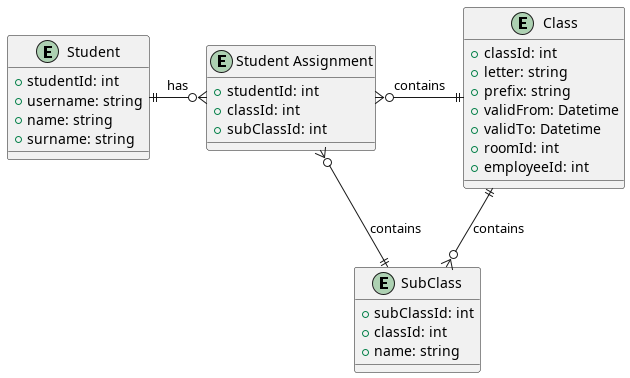
\includegraphics[width=\textwidth/2]{cd-student-assignment.png}
    \caption{Model tříd žákovských skupin}
    \label{fig:cd-student-assignment}
 \end{figure}

\subsection*{Databázový Model}

Databázový model musí zajistit, že všechny podmínky úplnosti, disjunkce a podmnožinové struktury jsou dodrženy. Toho lze dosáhnout pomocí správného nastavení cizích klíčů, unikátních omezení a triggerů.

\subsubsection*{Úplnost}

Úplnost zajišťuje, že každá třída je pokryta skupinami tak, aby žádný student nezůstal nezařazen. V aplikační logice zajistíme, že všechny skupiny dohromady pokrývají celou třídu. To můžeme kontrolovat při každém přiřazení studenta do skupiny. Je nezbytné, aby všechny skupiny třídy byly disjunktní a jejich sjednocení tvořilo celou třídu.

\subsubsection*{Disjunkce}

Disjunkci zajistíme na úrovni databáze pomocí unikátních omezení. Každý student může patřit pouze do jedné skupiny určitého typu v dané třídě. To lze implementovat pomocí unikátních indexů nebo pomocí aplikační logiky, která před přiřazením studenta do skupiny provede potřebné kontroly.

\subsubsection*{Podmnožinová struktura}

Podmnožinovou strukturu zajistíme pomocí cizích klíčů a referenční integrity. Každá skupina musí odkazovat na existující třídu a každé přiřazení studenta do skupiny musí odkazovat na existujícího studenta, třídu a skupinu.

\subsection*{Nejefektivnější řešení}

Pro zajištění úplné konzistence dat v databázi je nutné implementovat následující mechanismy.

\subsubsection*{Validace na úrovni aplikace}

Při každém přiřazení studenta do skupiny zkontrolujeme, zda přiřazení splňuje podmínky úplnosti a disjunkce. Pokud podmínky nejsou splněny, přiřazení se neprovede a uživatel obdrží příslušnou chybovou zprávu. Aplikační logika bude muset zohlednit také případy, kdy se celá třída učí společně a není třeba přiřazovat studenty do skupin.

\subsubsection*{Unikátní omezení}

Na úrovni databáze zavedeme unikátní omezení, která zajistí, že každý student může patřit pouze do jedné skupiny určitého typu v dané třídě. Tím zajistíme disjunkci dat.

\subsubsection*{Referenční integrita}

Pomocí cizích klíčů zajistíme, že každá skupina je podmnožinou existující třídy a každé přiřazení studenta odkazuje na existujícího studenta, třídu a skupinu. Tím zajistíme podmnožinovou strukturu.

\begin{figure}[H]
    \centering
    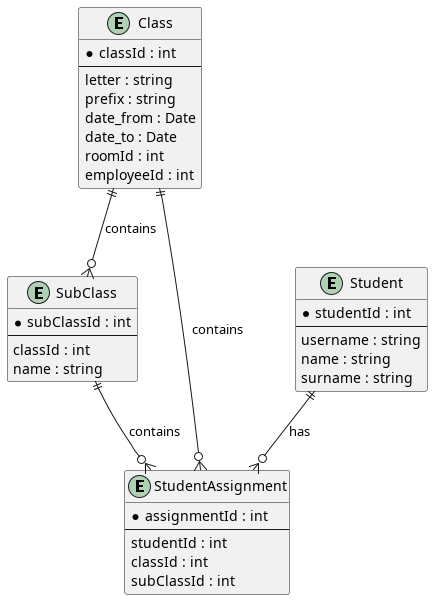
\includegraphics[width=\textwidth/2]{cd-referencni-identita.png}
    \caption{Referenční identita}
    \label{fig:cd-referencni-identita}
 \end{figure}

\subsection*{Diskuse o efektivitě řešení}

Implementace výše uvedených mechanismů v kombinaci s aplikační logikou poskytuje robustní řešení pro správu tříd a jejich skupin ve vzdělávacím systému. Validace na úrovni aplikace umožňuje flexibilitu a zajišťuje, že jsou splněny všechny matematické podmínky. Unikátní omezení a referenční integrita na úrovni databáze zajišťují konzistenci dat a minimalizují riziko chyb.

Tímto způsobem zajišťujeme:

\begin{itemize}
    \item \textbf{Úplnost}: Každá třída je kompletně pokryta skupinami a žádný student nezůstane nezařazen.
    \item \textbf{Disjunkce}: Každý student může být přiřazen pouze do jedné skupiny určitého typu v dané třídě.
    \item \textbf{Podmnožinová struktura}: Každá skupina je vždy podmnožinou konkrétní třídy, ke které patří.
\end{itemize}